\documentclass{article}
\usepackage[utf8]{inputenc}

\usepackage{float}
\usepackage{graphicx}
\usepackage{graphics}

\usepackage{subcaption}
\usepackage{caption}

\usepackage{amssymb}
\usepackage{amsmath}

\usepackage{multicol}
\usepackage{color}

\title{Numerical Work: Hawkes Processes in Limit Order Books}
\author{Aiden Huffman, Anatoliy Swishchuk}
\date{\today}

\begin{document}

\maketitle

\section*{Numerical Analysis}

In order to test the validity of our models and determine which best fits empirical data, we have considered level 1 LOB data for Apple, Amazon, Google, Microsoft and Intel on June 21st, 2012 [\textcolor{blue}{ref:LOBSTER}]. We first verify that the data is reasonable for our model but checking it's liquidity, this is illustrated in Table [\ref{table:liquidity}].

\begin{table}[htpb]
\centering
\begin{tabular}{c|c|c}

Ticker & Avg \# of Orders per Second & Price Changes in 1 Day\\
\hline
AAPL & 51 & 64,350\\
AMZN & 25 & 27,557\\
GOOG & 21 & 24,084\\
MSFT & 173 & 3,217\\
INTC & 176 & 4,060\\

\end{tabular}
\caption{\label{table:liquidity} Stock liquidity of AAPL, AMZN, GOOG, MSFT and INTC for June 21st, 2012.}
\end{table}

The high number of daily price changes suggests that we can use asymptotic analysis in order to approximate long-run volatility using order flow by finding the diffusion limit of the price process [\textcolor{blue}{ref:tyler - copied}]. Because we do not want to include opening and closing auctions we omit the first and last fifteen minutes of our data. We motivate the arrival process by analyzing the inter-arrival times and clustering to a ensure the arrival process is not Poisson and exhibits the characteristics of a Hawkes Process, this is illustrated in Figures [\ref{fig:poisson}] and [\ref{fig:clustering}].

Furthermore, the relationship between our diffusion coefficient and arrival process is limited to the expected number of arrivals on a unit interval. This implies that results for a simple exponential model can be easily generalized to a non-linear one. This makes it possible to work with a simplified model for our Hawkes process which is still rich enough to capture our observations. Keeping this in mind, we restrict ourselves to an exponential kernel and estimate parameters using a MLE [\textcolor{blue}{ref:laub}]. We provide these estimates in Table [\ref{table:params}] and compare the empirical expected number of arrivals and compare with the MLE estimate in Table [\ref{table:unitinterval}]

\begin{table}[htpb]

\centering
\begin{tabular}{c|c|c|c}
     &  $\lambda$ & $\alpha$ & $\beta$\\
\hline
AAPL & 1.4683 & 1045.2676 & 2556.1844\\
AMZN & 0.6443 & 653.7524 & 1556.1702\\
GOOG & 0.4985 & 865.8553 & 1980.4409\\
MSFT & 0.0659 &479.3482 & 908.0032\\
INTC & 0.0471 & 399.6389 & 760.4991
\end{tabular}

\caption{\label{table:params} Each parameter was estimated using a particle swarm optimization method in an attempt to globally optimize the negative log-likelihood function. The values for $\lambda$, $\alpha$ and $\beta$ for each data set are as provided.}
\end{table}

Obviously the MLE method accurately estimates the expected number of arrivals on the unit interval. This means we can confidently say for our data that our parameters will work reasonably with our models. We provide the estimated parameters in Table [\ref{table:params}]

\begin{table}[htpb]

\centering
\small

\begin{tabular}{ c | c | c }

 & Emp. $E[N([0,1])]$ & MLE\\
\hline
AAPL & 2.4840 & 2.4841\\

AMZN & 1.1110 & 1.1110\\

GOOG & 0.8857 & 0.8857\\

MSFT & 0.1395 & 0.1396\\

INTC & 0.0991 & 0.0992\\

\end{tabular}
\caption{\label{table:unitinterval} Expected number of arrivals on a unit interval using estimated parameters from an MLE method is compared against the empirical arrivals.}
\end{table}

\subsection*{CHPDO}

We first consider a compound Hawkes process with dependent orders, namely
\begin{equation}
    S_t = S_0 + \sum_{k=1}^{N(t)}X_k
\end{equation}
where $X_k\in\{+\delta, -\delta\}$ is a continuous-time two state Markov chain, $\delta$ is of fixed size and $N(t)$ is the number of mid price movements up to time $t$ described by a Hawkes process.

We have opted to study the mid price changes of our model. Thus $S_t$ can be computed by averaging the best bid and ask price. Noting that the price is recorded in cents the smallest possible jump in the mid price is a half a cent which we will use as $\delta$. Furthermore, in order to estimate the transition matrix for the Markov chain $X_k$ we count the absolute frequencies of upward and downward price movements and from this calculate the relative frequencies giving an estimate for $p_{uu}$ and $p_{dd}$ which represent the conditional probabilities of an up/down movement given an up/down movement. Later we will consider several different sizes of mid price movements and will work with the convention that each movement will be assigned a state based off of its ordering in the reals. In this case, $-\delta$ will be state one, and $\delta$ with be state two. This results in the transition matrix $P$ given below.

\[P =
\begin{bmatrix}
p_{dd} & 1-p_{dd}\\
1-p_{uu} & p_{uu}
\end{bmatrix}
\]

After determining our parameters and transition probabilities we calculate $a^*$ and $\sigma$ in Table [\ref{table:chpdo_coeff}] together with $p_{uu}$ and $p_{dd}$.

\begin{table}[htpb]

\centering
\small

\begin{tabular}{ c | c | c | c | c }

 & $p_{dd}$ & $p_{uu}$ & $\sigma$ & $a^*$\\
\hline
AAPL & 0.4956 & 0.4933 & 0.0049 & -1.1463e-5\\

AMZN & 0.4635 & 0.4576 & 0.0046 & -2.7373e-5\\

GOOG & 0.4769 & 0.4461 & 0.0046 & -1.4301e-4\\

MSFT & 0.6269 & 0.5827 & 0.0062 & -2.7956e-4\\

INTC & 0.6106 & 0.5588 & 0.0059 & -3.1185e-4\\

\end{tabular}

\caption{ \label{table:chpdo_coeff} Provided above are the values for $s^*$, $\sigma$ as well as the probabilities of an upward/downward movement given an upward/downward movement for each of the 5 stocks in question.}
\end{table}

Provided these values we can test our claim that our model accurately describes the mid price process satisfies we will use the diffusion limit proved earier, namely
\begin{equation}
    \frac{S_{nt} - N(nt)a^*}{\sqrt{n}}\xrightarrow{n\to\infty} \sigma\sqrt{\frac{\lambda}{1-\alpha/\beta}}W(t).
\end{equation}
If the data satisfies our proposed model then when considering large windows of time (5min, 10min, 20min), then when we would expect to see the empirical and theoretical standard deviations to follow each other closely. To test this we compare the equivalent process, constructed by multiplying the LHS and RHS by $\sqrt{n}$. Then cutting our data into disjoint windows of size $n$, specifically $[in, (i+1)n]$ with $t = 1$ and by setting the left bound as our starting time we can calculate $S_{nt} - N(nt)a^*$ for each individual window and give a generalized formula for this below.
\begin{equation}\label{eq:S_star}
    S^*_{i} = S_{(i+1)nt} - S_{int} - (N((i+1)nt) - N(int))a^*
\end{equation}
 This gives a collection of values $\{S^*_i\}$ over which we compute the standard deviation. If our model is accurate would would expect that 
 \begin{equation}
    \text{std}\{S^*_i\} \approx \sqrt{nt}\sigma\sqrt{\frac{\lambda}{1-\alpha/\beta}},\ \text{where } t = 1.
 \end{equation}
 We plot the empirical standard deviation against the theoretical one for various window sizes starting at 10 seconds and increasing in steps of 10 seconds until we reach 20 minutes, this is illustrated in Figure [\ref{fig:chpdofit}].

Several important remarks should be made at this point. It is clear that while the model accurately predicts the overall trend for MSFT and INTC, we severely underestimate the variability in the mid price process for APPL, AMZN and GOOG. Furthermore, as the window size increases the overall spread in the data increases. We attribute this to the decreasing sample size imposed on us as we increase the window size. For example when we consider a 20 minute window, we can only construct 27 disjoint windows in the 9 hour trading day forcing us to deal with the problem of predicting a 'population' standard deviation from a increasingly small sample. We remedy this by using a variance stabilizing transformation in later sections. Specifically, a popular method for a Poisson process is to take the square root of our empirical and theoretical standard deviations. This makes it possible to see the overall trend in the data better and gain a clearer idea of goodness of fit from there.

\subsection*{GCHP2SDO}

As of now we have considered a fixed delta related to the trading tick size. However, if we consider the mid price changes for APPL, AMZN and GOOG the assumption of a fixed tick size is violated. In fact, we observe that approximately approximately 61\%, 53\% and 71\% of all mid price changes are larger than half a tick size, which is opposed to what we observe for MSFT and INTC where all mid price changes occur at the half tick size, we illustrate this for AAPL, AMZN and GOOG in Figure [\ref{fig:tickhist}].

It is clear in Figure [\ref{fig:tickhist}] additional considerations need to be made. A simple way to include the variability in mid price movements in our model is to introduce $a(X_i)$ as described in [\textcolor{blue}{eq:GCHP2SDO}]. It is of course necessary to determine the values of $a( \cdot )$ for each state of our Markov chain. A naive method is to take the mean of the downward and upward mid price movements and assign them to $a(1)$ and $a(2)$ respectively. We provide these values in Table [\ref{table:2sdoticks}].

\begin{table}[htpb]

\centering
\begin{tabular}{c|c|c}
     &  $a(1)$ & $a(2)$\\
\hline
AAPL & -0.0172 & 0.0170\\
\hline
AMZN & -0.0134 & 0.0133\\
\hline
GOOG & -0.0302 & 0.0308\\
\end{tabular}

\caption{\label{table:2sdoticks} $a(i)$ is the average of the upward or downward mid price movements. Following our previous convention, the first state will be associated with the mean of all downward mid price movements and the second state will be associated with the mean of all upward mid price movements.}
\end{table}

In this step we have only endeavoured to better realize the actual price movements in our data. Therefore, when we observe a downward mid price movement we continue to assign it to state one and similarly for an upward price movement we continue to assign it to state two. It follows that our transition matrix will remain the same. Then using these new state values we recalculate $a^*$ and $\sigma$, providing them in Table [\ref{table:2SDO_coeff}]. The effect of these changes is investigated in Figure [\ref{fig:2SDOfit}]. Note that in Figure [\ref{fig:2SDOfit}] we have used the variance stabilizing transformation discussed earlier in order to better see the overall trend in our data.

\begin{table}[htpb]

\centering
\small

\begin{tabular}{ c | c | c | c | c }
 & $p_{dd}$ & $p_{uu}$ & $\sigma$ & $a^*$\\
\hline
AAPL & 0.4956 & 0.4933 & 0.0169 & -1.5624e-4\\
AMZN & 0.4635 & 0.4576 & 0.0123 & -1.0475e-4\\
GOOG & 0.4769 & 0.4461 & 0.0282 & -5.5095e-4\\
\end{tabular}

\caption{\label{table:2SDO_coeff} We above the values for $s^*$, $\sigma$ as well as the probabilities of an upwards/downwards movement given an upwards/downwards movement for the 3 stocks of interest.}
\end{table}

We see a significant improvement in the fits for AAPL and GOOG but the variability in mid price movements for AMZN is still underestimated by our model. The unexplained variance may be captured by investigating an n-state Markov chain since the additional transition probabilities could explain the variability missing in the 2-state case. [\textcolor{blue}{Motivate N-state process more}]

\subsection*{GCHPNSDO}

We introduce the N-state model described in Eq. [\textcolor{blue}{GCHPNSDO EQ}]. The immediate question becomes how best to choose the state values. We modify the quantile based approach from [\textcolor{blue}{ref:tyler}] [\textcolor{blue}{Can we motivate this?}]. After calculating the mid price changes we separate the data into upward and downward price movements. Then we calculate evenly distributed quantiles for both data sets. Depending on the data, several quantiles may be identical, we reject any duplicates. We thus obtain a list of bounds which we complete by adding the minimum observed value if necessary.

To determine the state values $a(X_i)$, we take the average of all mid price changes located between two neighbouring boundary values. Furthermore, we assign a mid price change to state $i$ if it is greater than or equal to the $(i-1)$th boundary and strictly less than the $i$th boundary. An exception is made for the largest upper bound where equality is permitted at both ends.

As we could not capture the full variability of mid price changes for AMZN before. In this case for tractability we consider 14 boundary values to generate a 12-state Markov chain. Instead of providing the transition matrix, we provide the ergodic probabilities for the transition matrix and the associated states in Table [\ref{table:AMZN_data}].
\begin{table}[htpb]

\centering
\small
\textbf{AMZN}

\vspace{\baselineskip}

\begin{tabular}{ c | c | c }
 & $\pi_i^*$ & $a(X_i)$\\
\hline
1 & 0.0384 & -0.0475\\
2 & 0.0172 & -0.0300\\
3 & 0.0264 & -0.0250\\
4 & 0.0382 & -0.0200\\
5 & 0.0576 & -0.0150\\
6 & 0.3249 & -0.0064\\
7 & 0.2321 & 0.0050\\
8 & 0.0923 & 0.0100\\
9 & 0.0578 & 0.0150\\
10 & 0.0353 & 0.0200\\
11 & 0.0412 & 0.0271\\
12 & 0.0387 & 0.0476
\end{tabular}

\caption{\label{table:AMZN_data} Above we have provide the state, associated ergodic probabilities and state values $a(i)$ for AMZN, given a 12 state Markov chain.}
\end{table}
In order to compare the two state and N-state approaches we first take a qualitative approach and plot the two theoretical and empirical standard deviations against each other. Then we take the mean of the residuals for each point to gain a better quantitative understanding of the overall improvement.

\subsection*{Conclusion}

It is clear that while our model does visually appear to fit the expected variability with significant precision, it still fails to capture the complete dynamics of mid price changes such in the case of AMZN. Regardless, when we investigate the mean residuals for AAPL and GOOG we see the N-state case can still improve our results from the two state case. We constructed a 17 state Markov chain for AAPL, which resulted in a mean residual of $0.0036$ which is approximately a 28\% improvement to the two state case where the mean residual was $0.0050$. Even more extreme, using a 25 state Markov chain for GOOG which resulted in a mean residual of $0.0046$ which is a 60\% improvement from the two state case with a mean residual of $0.0115$. We conclude with Table [\ref{table:meanres}] which provides the mean residuals for AAPL, AMZN and GOOG with several of Markov chains of varying numbers of states. We also include mean residuals for INTC and MSFT in the two state case.

\begin{table}[htpb]
    \centering
    \begin{tabular}{c|c|c|c|c|c}
     & CHPDO & 2 & 8 & 16 & 32\\
    \hline
    AAPL & 0.2679 & 0.0050 & 0.0036 & 0.0036 & 0.0036\\
    AMZN & 0.1122 & 0.0208 & 0.0131 & 0.0124 & 0.0123\\
    GOOG & 0.4036 & 0.0115 & 0.0048 & 0.0045 & 0.0047\\
    INTC & 1.7917e-5 & * & * & * & *\\
    MSFT & 1.0586e-4 & * & * & * & *
    \end{tabular}
    \caption{\label{table:meanres} We list the mean residuals for several Markov chains with varying numbers of states. These were generated using our modified quantile approach choosing 2, 8, 16 or 32 quantiles. We see that in general the mean residual decreases to some lower limit where we can no longer perform any better. Furthermore we place *'s for INTC and MSFT since their calculations can not result in a better mean residual. This should be clear as the only observed mid price changes were a half tick size and therefore the only unique quantiles will be the same as the CHPDO case.}
    
\end{table}

\newpage

\begin{figure}[htbp]

\centering
\begin{subfigure}[t]{0.49\textwidth}
\captionsetup{labelformat=empty}

\caption{\textbf{AAPL}}
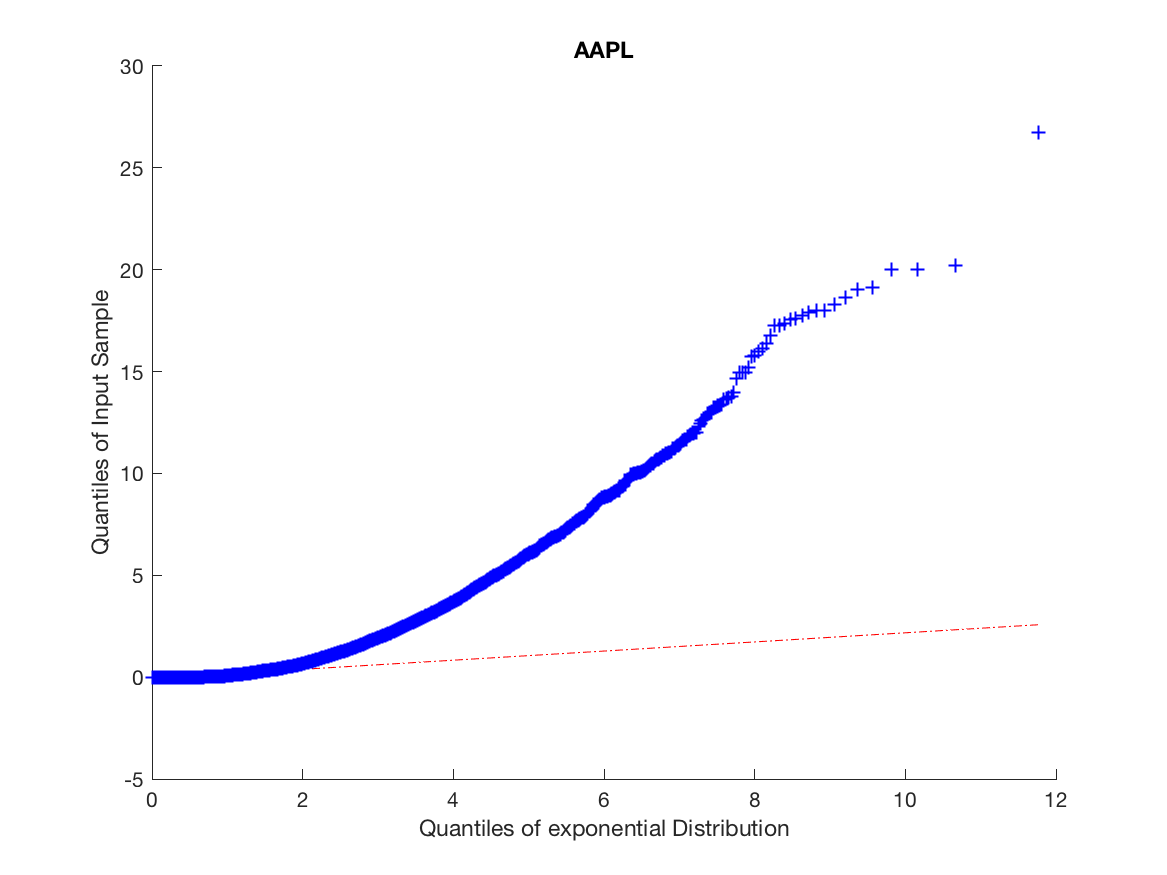
\includegraphics[width=\textwidth, trim = 0 0 0 30, clip]{QQ_Plots/AAPL_QQ.png}

\end{subfigure}
\begin{subfigure}[t]{0.49\textwidth}
\captionsetup{labelformat=empty}

\caption{\textbf{AMZN}}
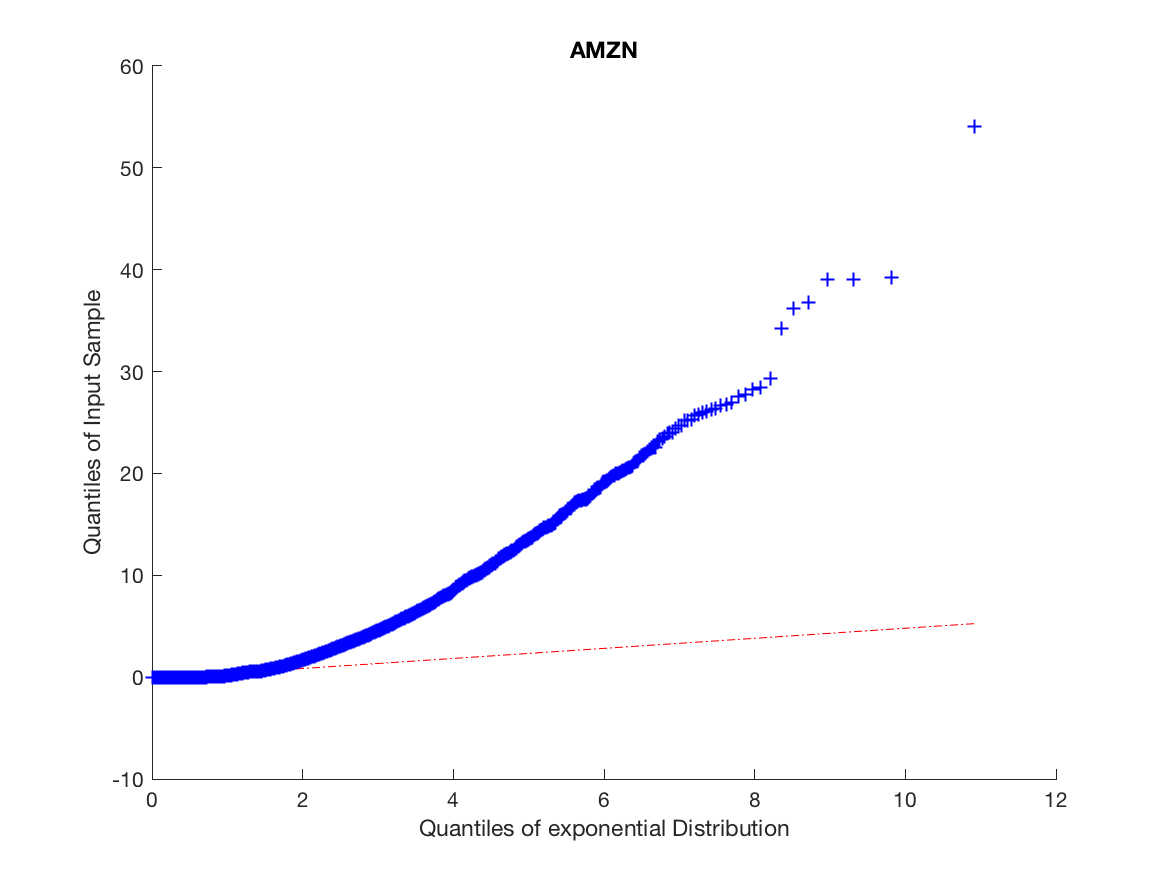
\includegraphics[width=\textwidth, trim = 0 0 0 30, clip]{QQ_Plots/AMZN_QQ.png}
\end{subfigure}

\vspace{3mm}

\begin{subfigure}[t]{0.49\textwidth}
\captionsetup{labelformat=empty}

\caption{\textbf{GOOG}}
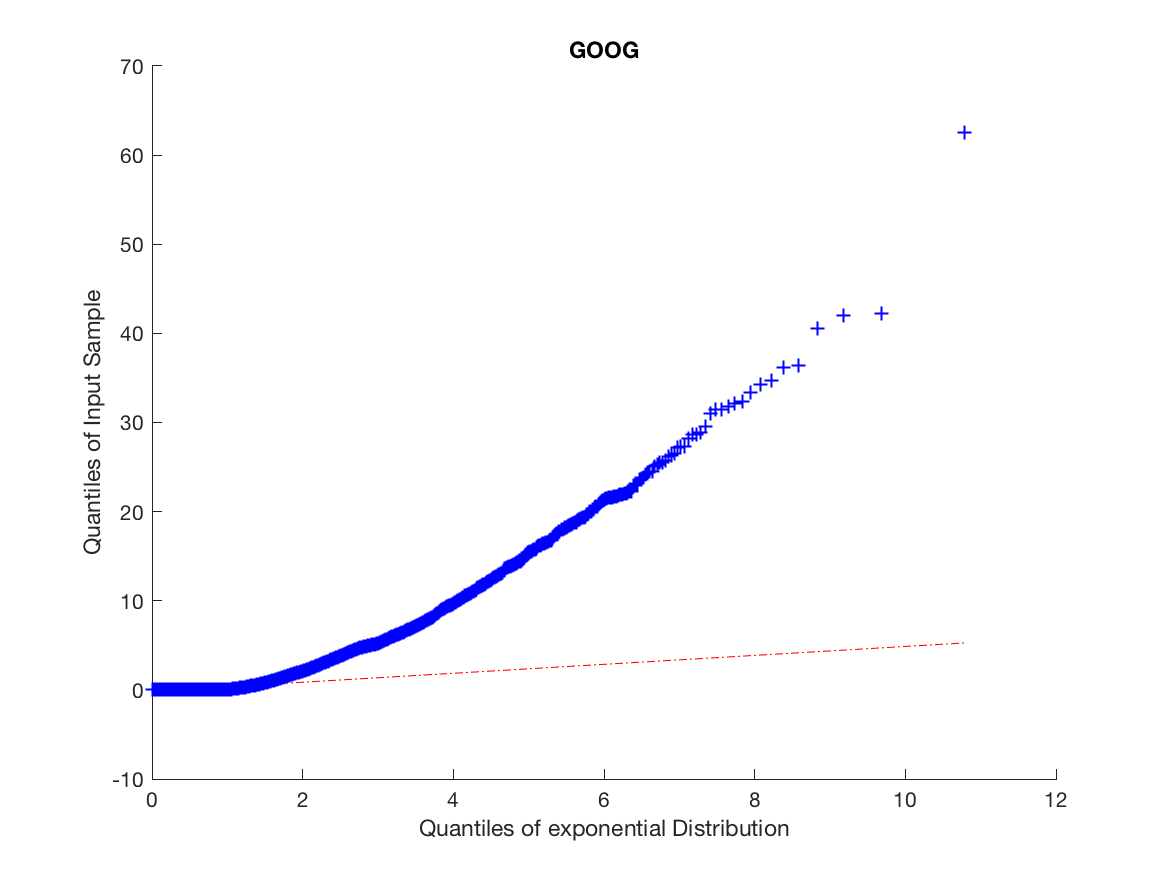
\includegraphics[width=\textwidth, trim = 0 0 0 30, clip]{QQ_Plots/GOOG_QQ.png}

\end{subfigure}
\begin{subfigure}[t]{0.49\textwidth}
\captionsetup{labelformat=empty}

\caption{\textbf{INTC}}
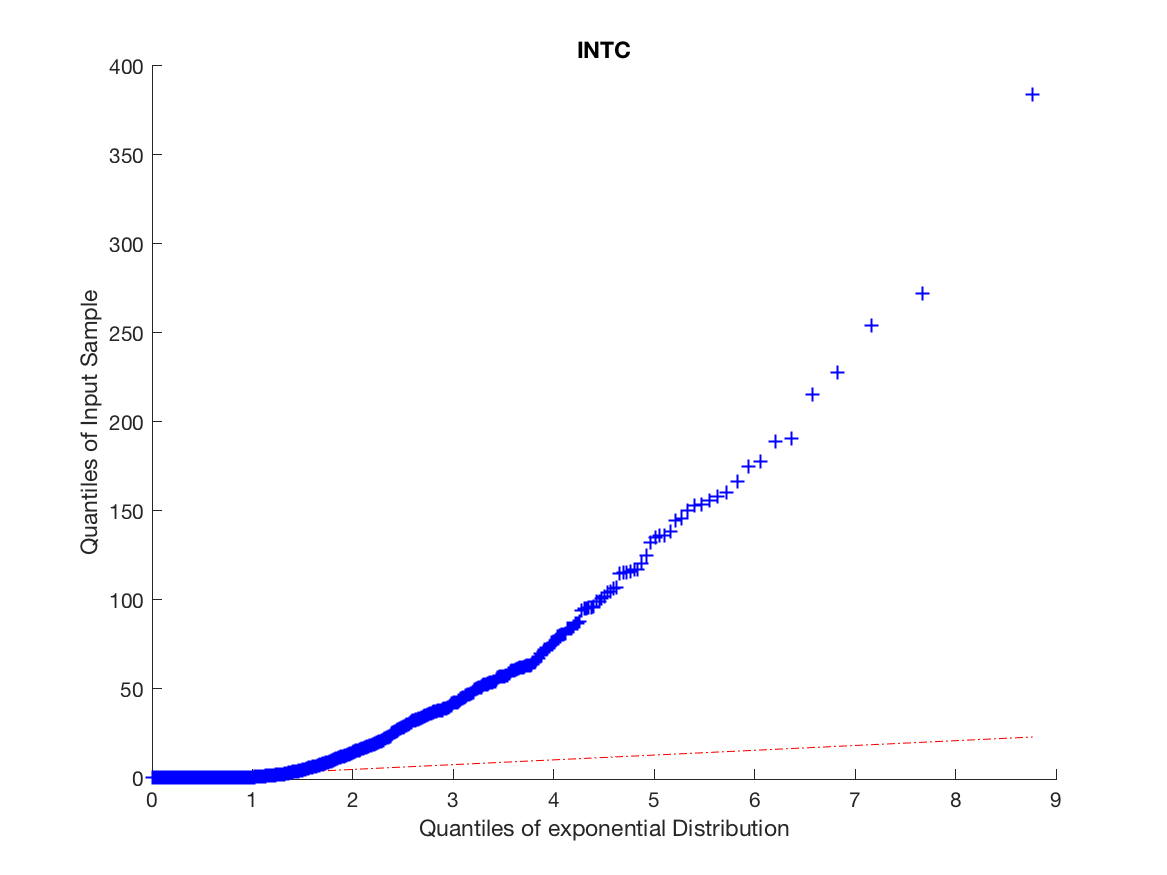
\includegraphics[width=\textwidth, trim = 0 0 0 30, clip]{QQ_Plots/INTC_QQ.png}
\end{subfigure}

\vspace{3mm}

\begin{subfigure}[t]{0.49\textwidth}
\captionsetup{labelformat=empty}

\caption{\textbf{MSFT}}
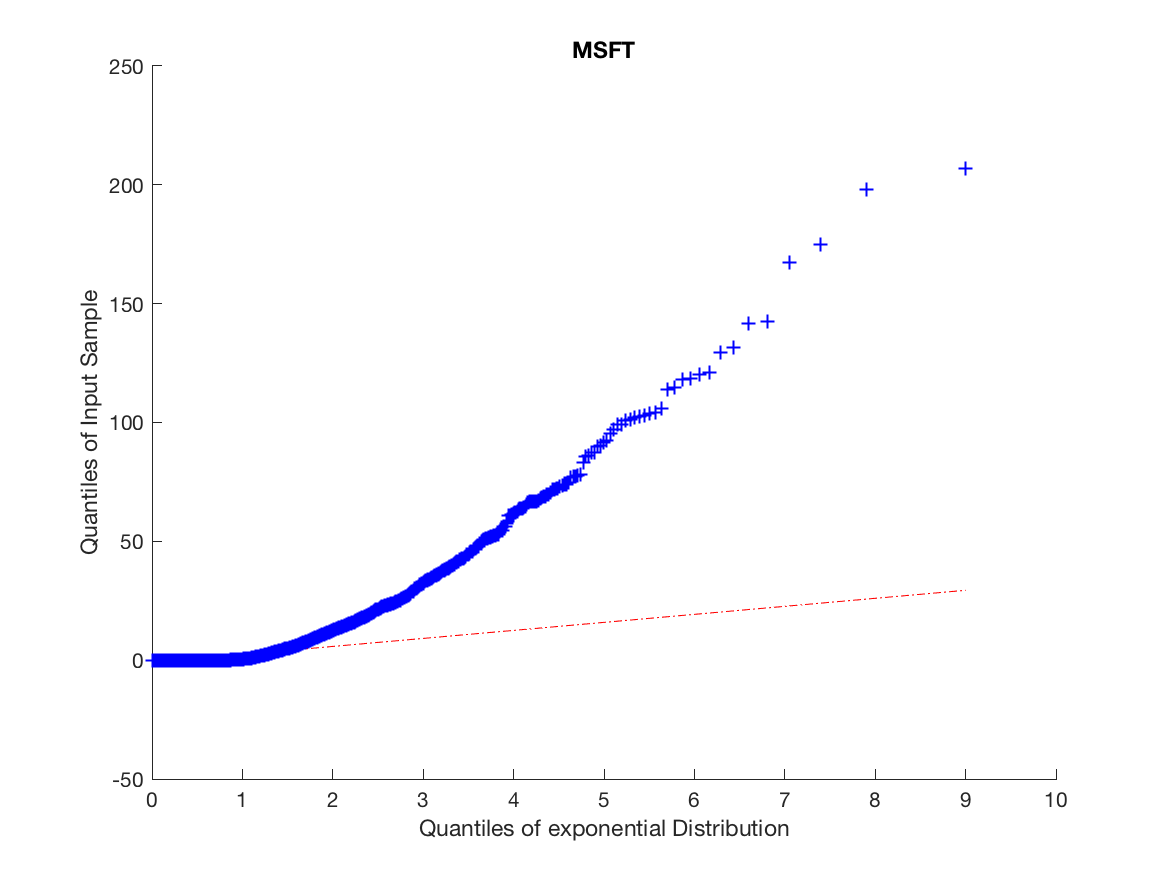
\includegraphics[width=\textwidth, trim = 0 0 0 30, clip]{QQ_Plots/MSFT_QQ.png}
\end{subfigure}

\caption{\label{fig:poisson} Above we provide a quantile-quantile plot of our empirical inter-arrival times against a Poisson process for each of the five stocks. We see that the inter-arrival data does not fit the expected curve, providing evidence that the underlying arrival process is not Poisson.}
\end{figure}

\begin{figure}[htbp]

\centering
\begin{subfigure}[t]{0.49\textwidth}
\captionsetup{labelformat=empty}

\caption{\textbf{AAPL}}
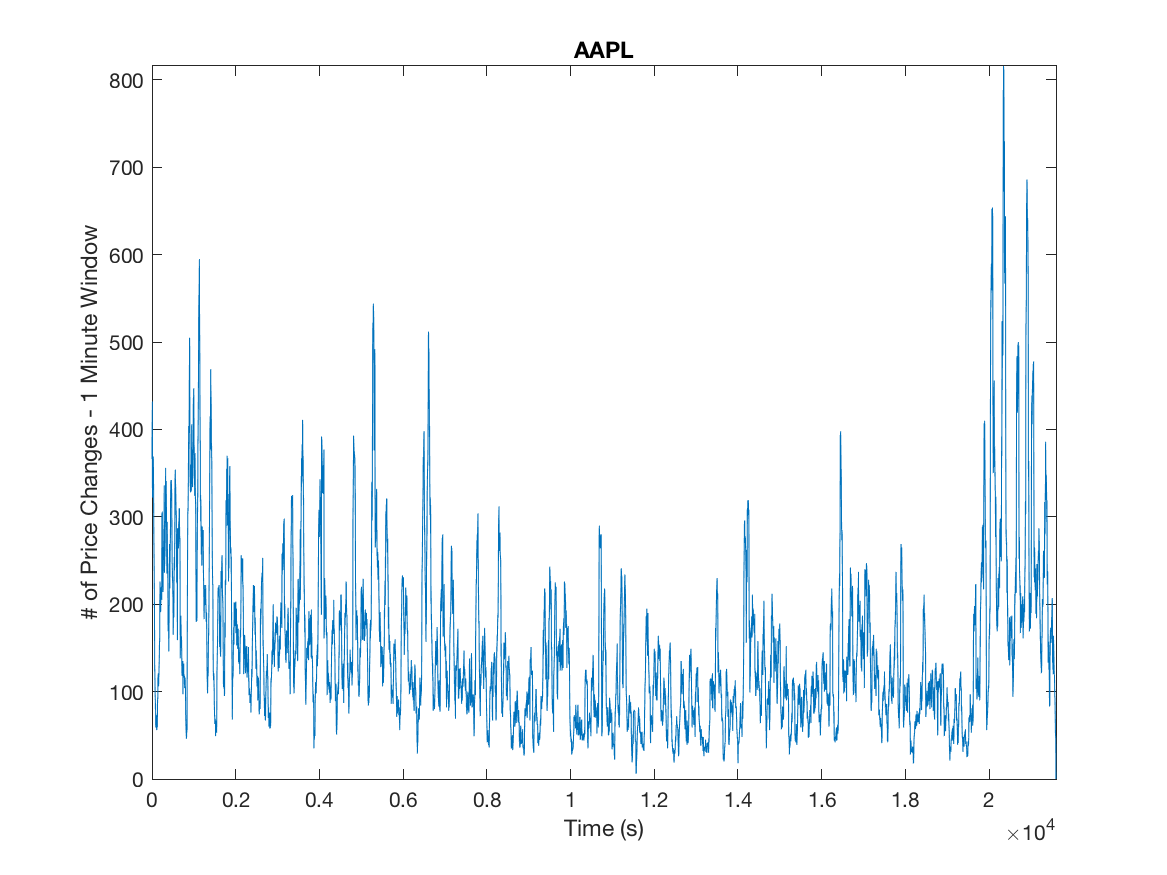
\includegraphics[width=\textwidth, trim = 0 0 0 30, clip]{Cluster_Plots/AAPL_cluster.png}

\end{subfigure}
\begin{subfigure}[t]{0.49\textwidth}
\captionsetup{labelformat=empty}

\caption{\textbf{AMZN}}
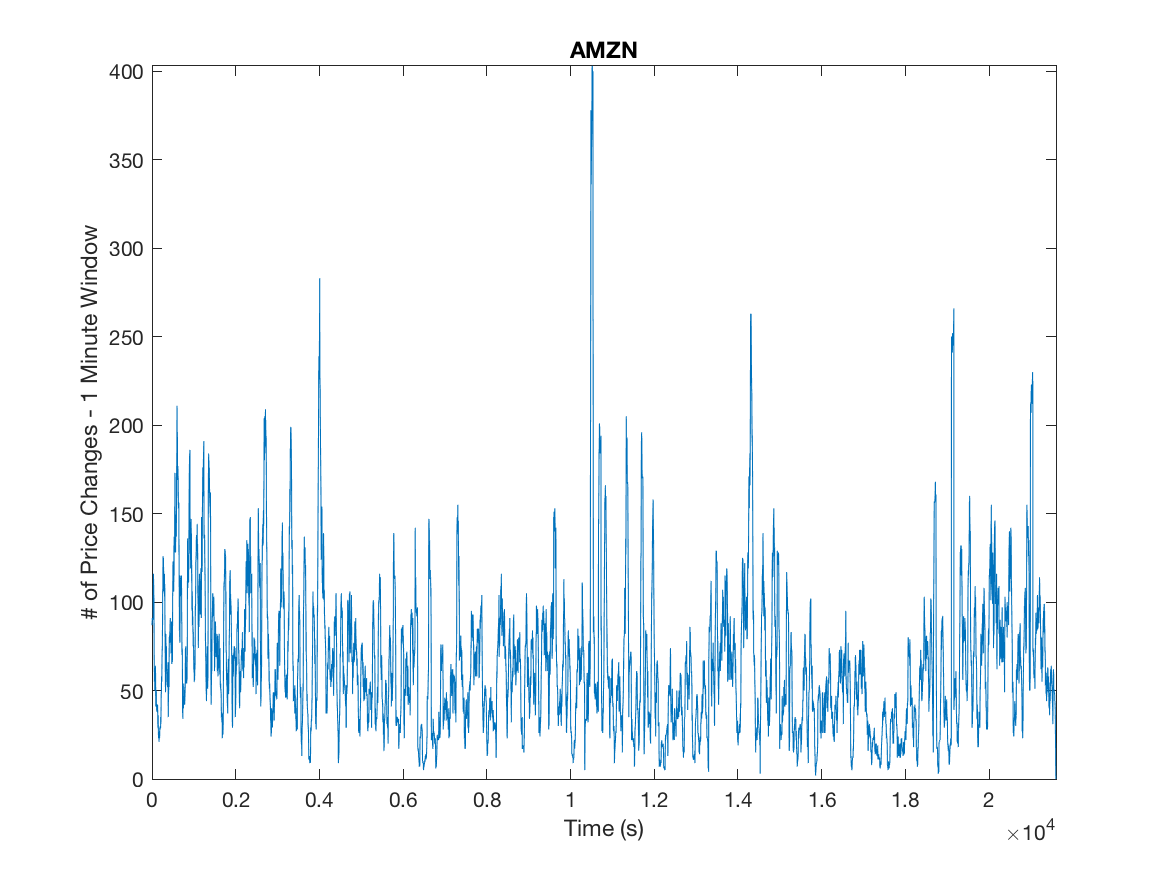
\includegraphics[width=\textwidth, trim = 0 0 0 30, clip]{Cluster_Plots/AMZN_cluster.png}
\end{subfigure}

\vspace{3mm}

\begin{subfigure}[t]{0.49\textwidth}
\captionsetup{labelformat=empty}

\caption{\textbf{GOOG}}
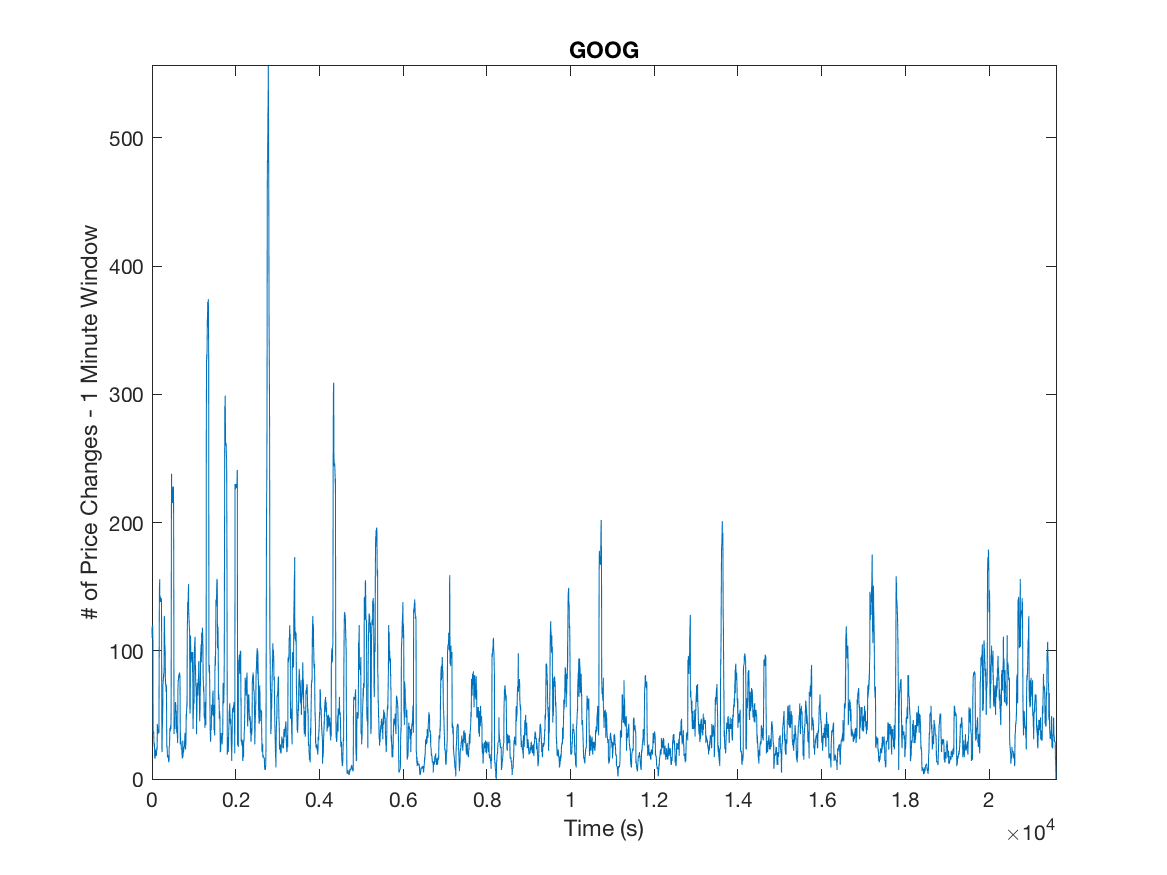
\includegraphics[width=\textwidth, trim = 0 0 0 30, clip]{Cluster_Plots/GOOG_cluster.png}

\end{subfigure}
\begin{subfigure}[t]{0.49\textwidth}
\captionsetup{labelformat=empty}

\caption{\textbf{INTC}}
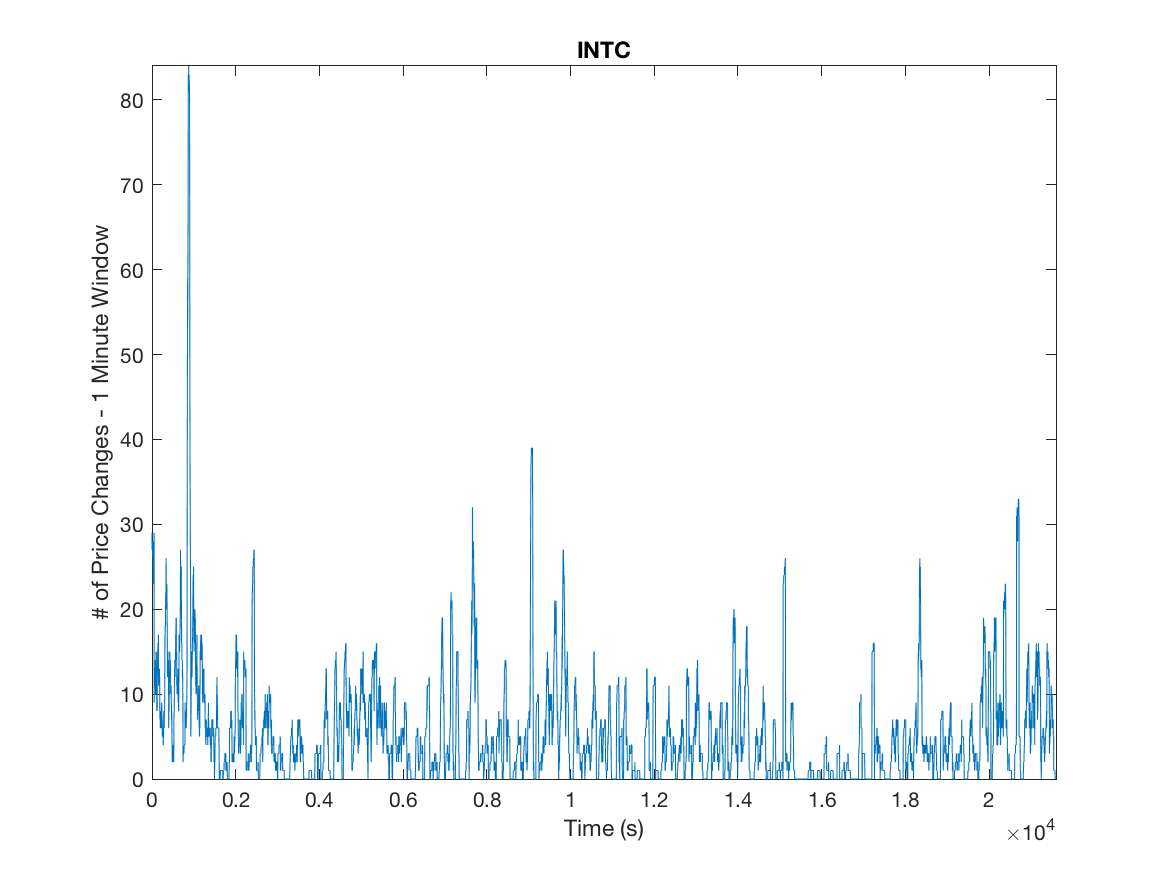
\includegraphics[width=\textwidth, trim = 0 0 0 30, clip]{Cluster_Plots/INTC_cluster.png}
\end{subfigure}

\vspace{3mm}

\begin{subfigure}[t]{0.49\textwidth}
\captionsetup{labelformat=empty}

\caption{MSFT}
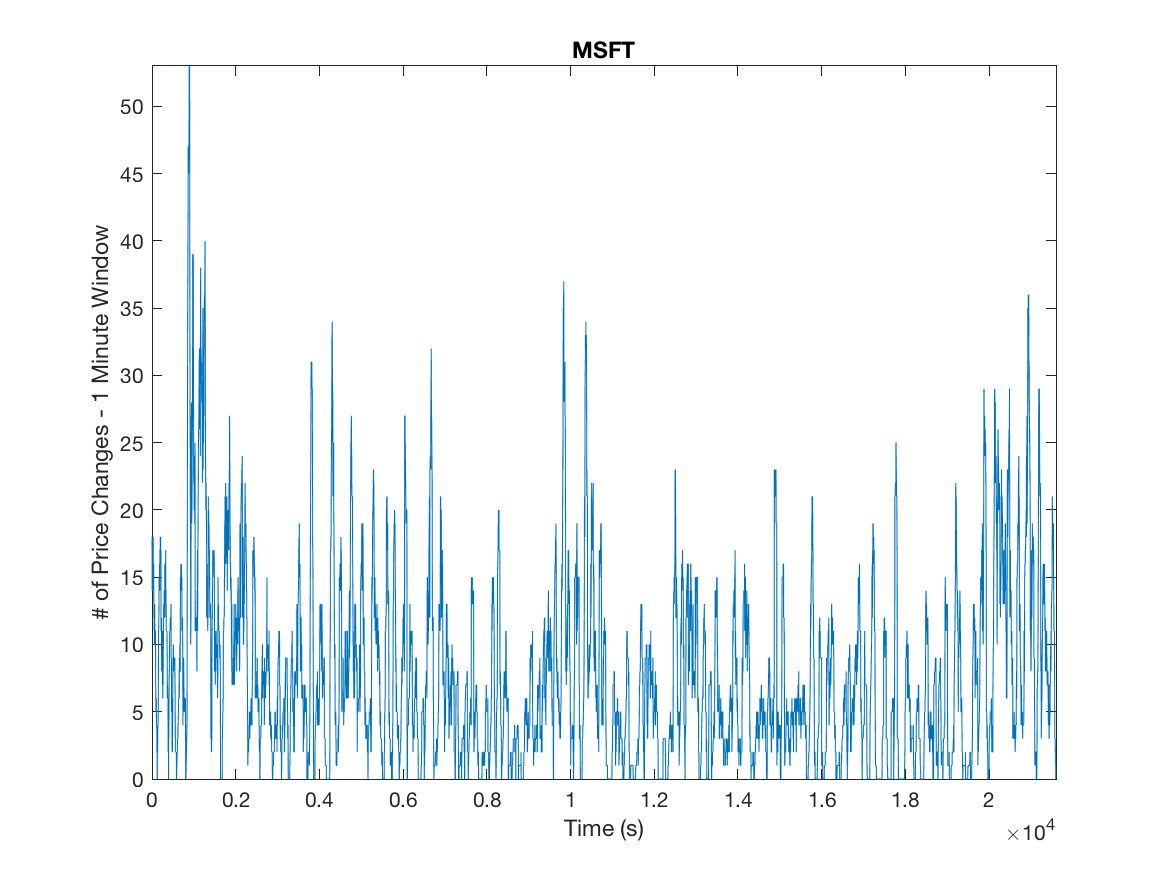
\includegraphics[width=\textwidth, trim = 0 0 0 30, clip]{Cluster_Plots/MSFT_cluster.png}
\end{subfigure}

\caption{\label{fig:clustering} Each plot shows the number of arrivals for a moving one minute window. From this we can conclude that there is a significant amount of clustering in the arrival of mid price changes, motivating the Hawkes model of our arrival process.}
\end{figure}

\begin{figure}[htbp]

\centering
\begin{subfigure}[t]{0.49\textwidth}
\captionsetup{labelformat=empty}

\caption{\textbf{AAPL}}
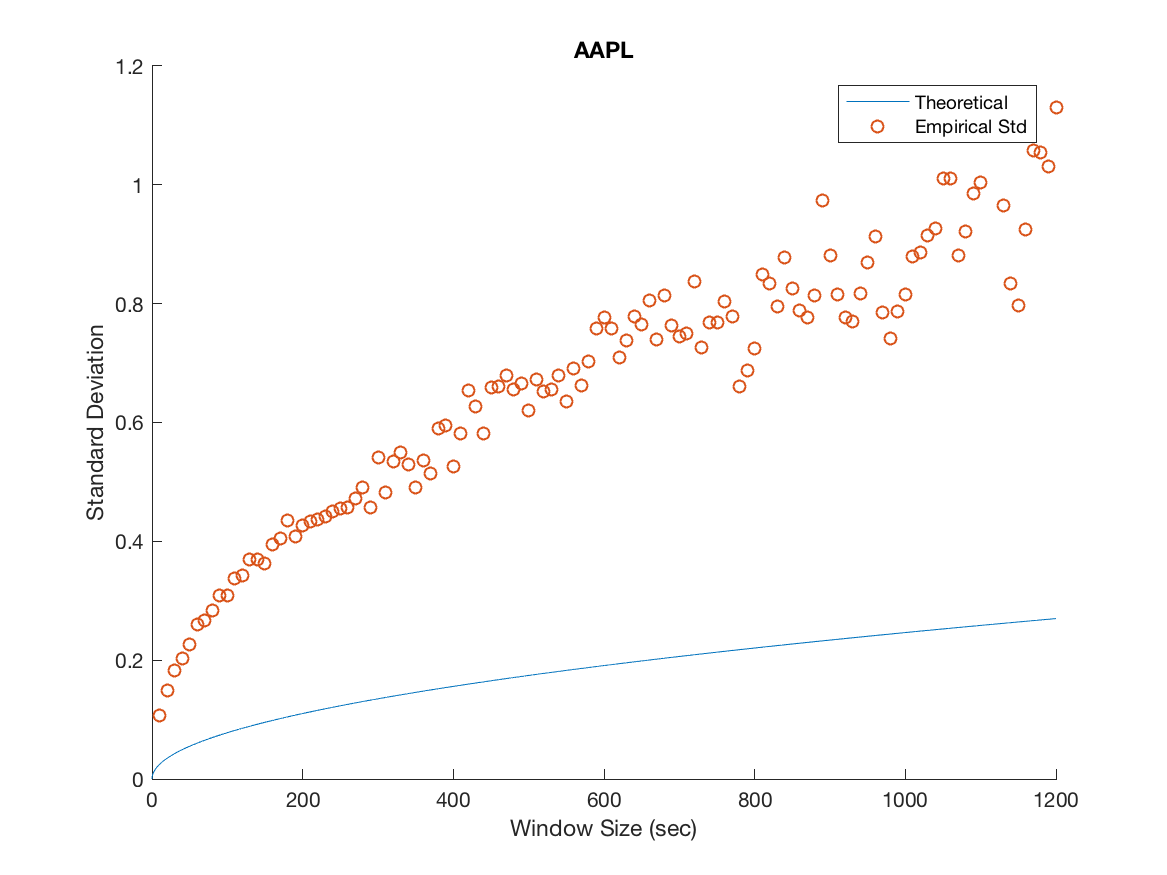
\includegraphics[width=\textwidth, trim = 0 0 0 30, clip]{CHPDO_Fit/AAPL_Plot_CHPDO_21600.png}

\end{subfigure}
\begin{subfigure}[t]{0.49\textwidth}
\captionsetup{labelformat=empty}

\caption{\textbf{AMZN}}
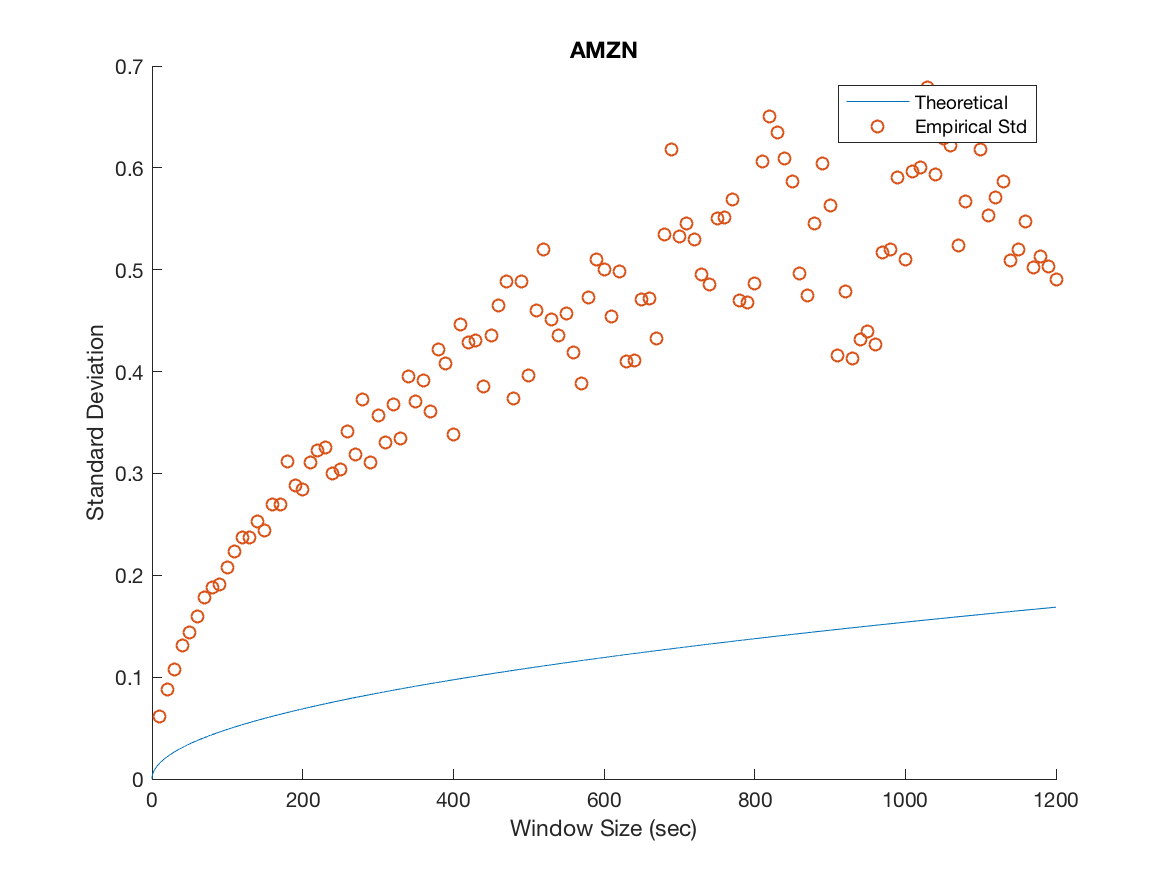
\includegraphics[width=\textwidth, trim = 0 0 0 30, clip]{CHPDO_Fit/AMZN_Plot_CHPDO_21600.png}
\end{subfigure}

\vspace{3mm}

\begin{subfigure}[t]{0.49\textwidth}
\captionsetup{labelformat=empty}

\caption{\textbf{GOOG}}
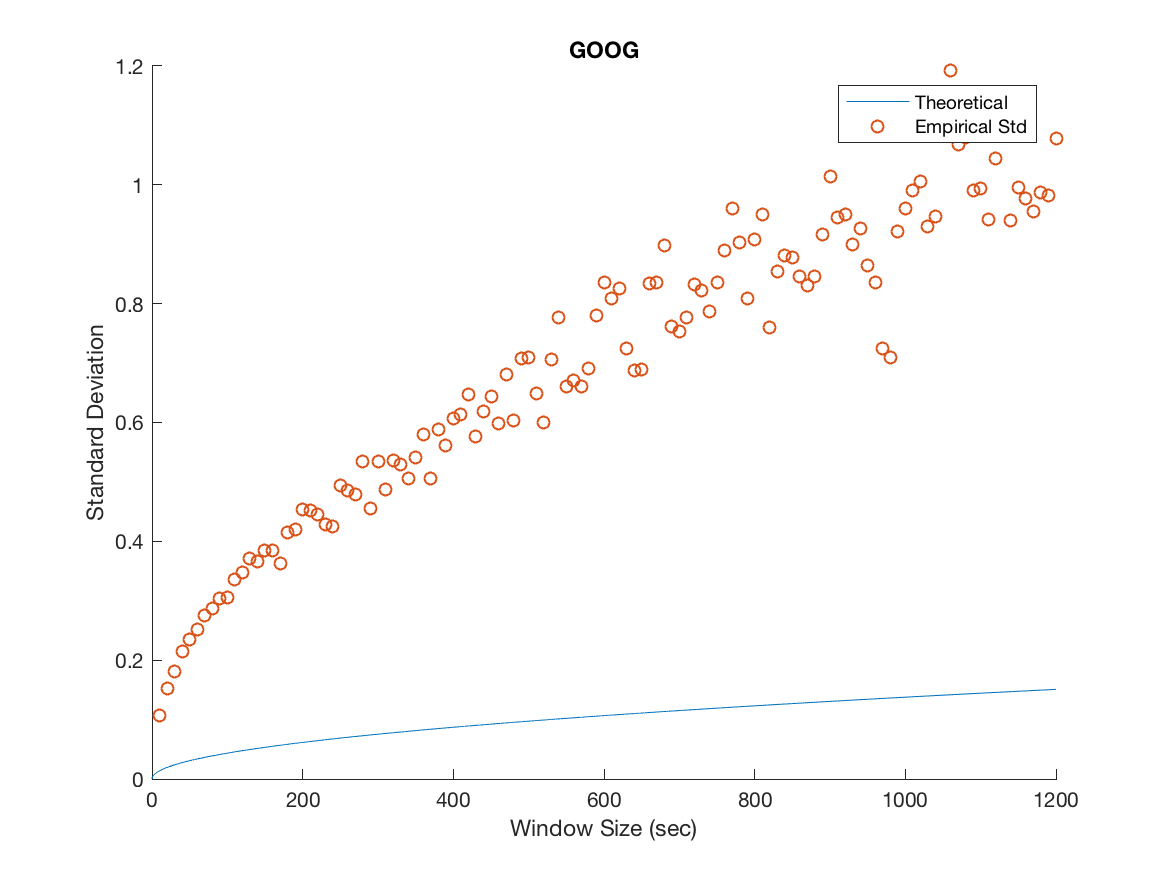
\includegraphics[width=\textwidth, trim = 0 0 0 30, clip]{CHPDO_Fit/GOOG_Plot_CHPDO_21600.png}

\end{subfigure}
\begin{subfigure}[t]{0.49\textwidth}
\captionsetup{labelformat=empty}

\caption{\textbf{INTC}}
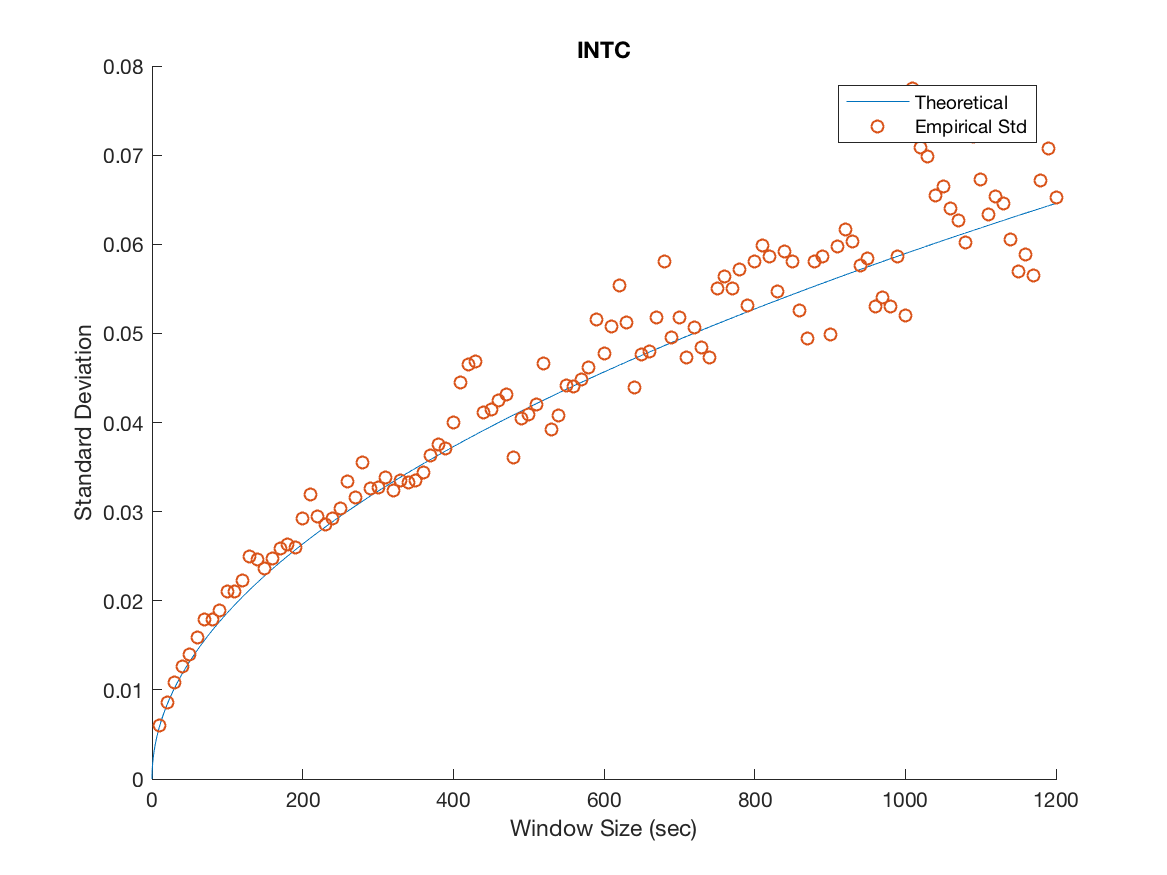
\includegraphics[width=\textwidth, trim = 0 0 0 30, clip]{CHPDO_Fit/INTC_Plot_CHPDO_21600.png}
\end{subfigure}

\vspace{3mm}

\begin{subfigure}[t]{0.49\textwidth}
\captionsetup{labelformat=empty}

\caption{MSFT}
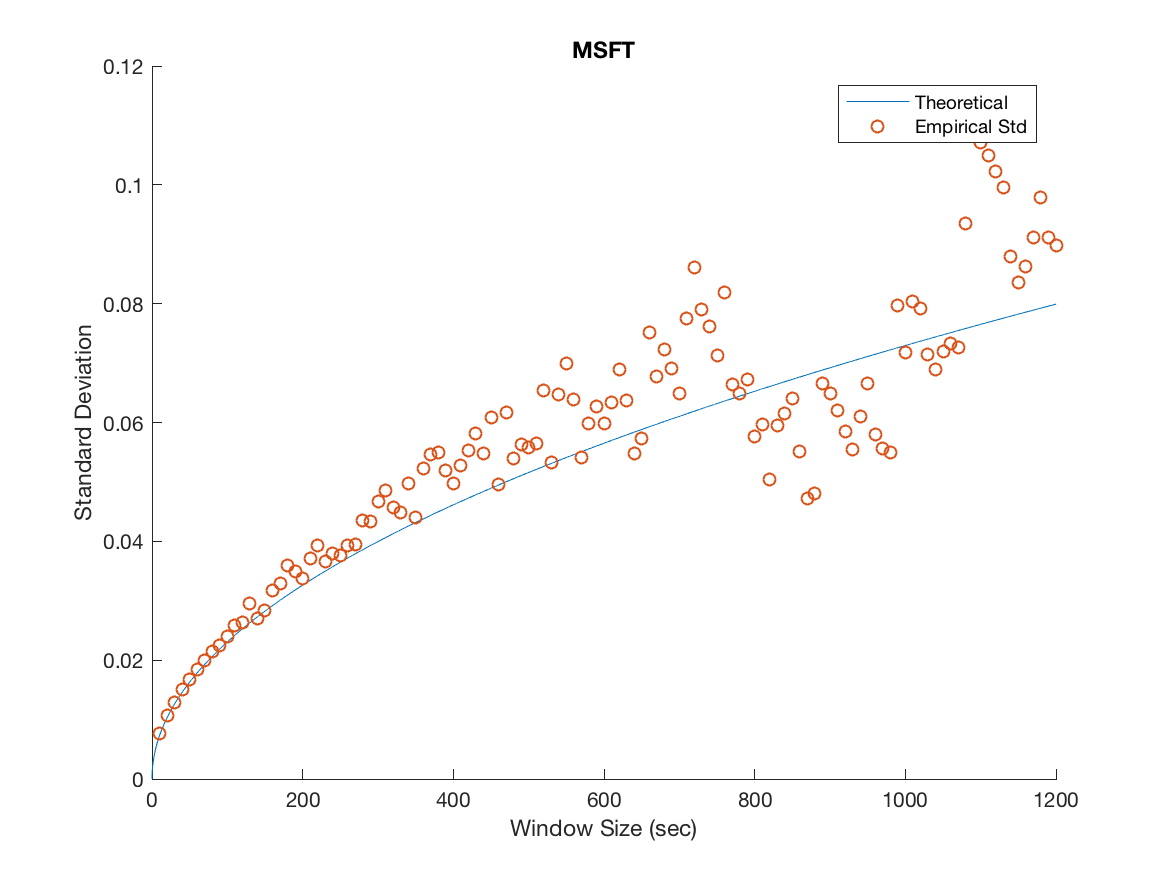
\includegraphics[width=\textwidth, trim = 0 0 0 30, clip]{CHPDO_Fit/MSFT_Plot_CHPDO_21600.png}
\end{subfigure}

\caption{\label{fig:chpdofit} Each figure compares the empirical standard deviation for a fixed window size to the theoretical standard deviation. We have plotted an empirical standard deviation for all $n$ from 10 seconds to 20 minutes in step sizes of 10 seconds. Each empirical standard deviation corresponds to a single point in the scatter plot and the plotted curve corresponds to the predicted theoretical value.}


\end{figure}

\begin{figure}[htbp]

\centering
\begin{subfigure}[t]{0.49\textwidth}
\captionsetup{labelformat=empty}

\caption{\textbf{AAPL}}
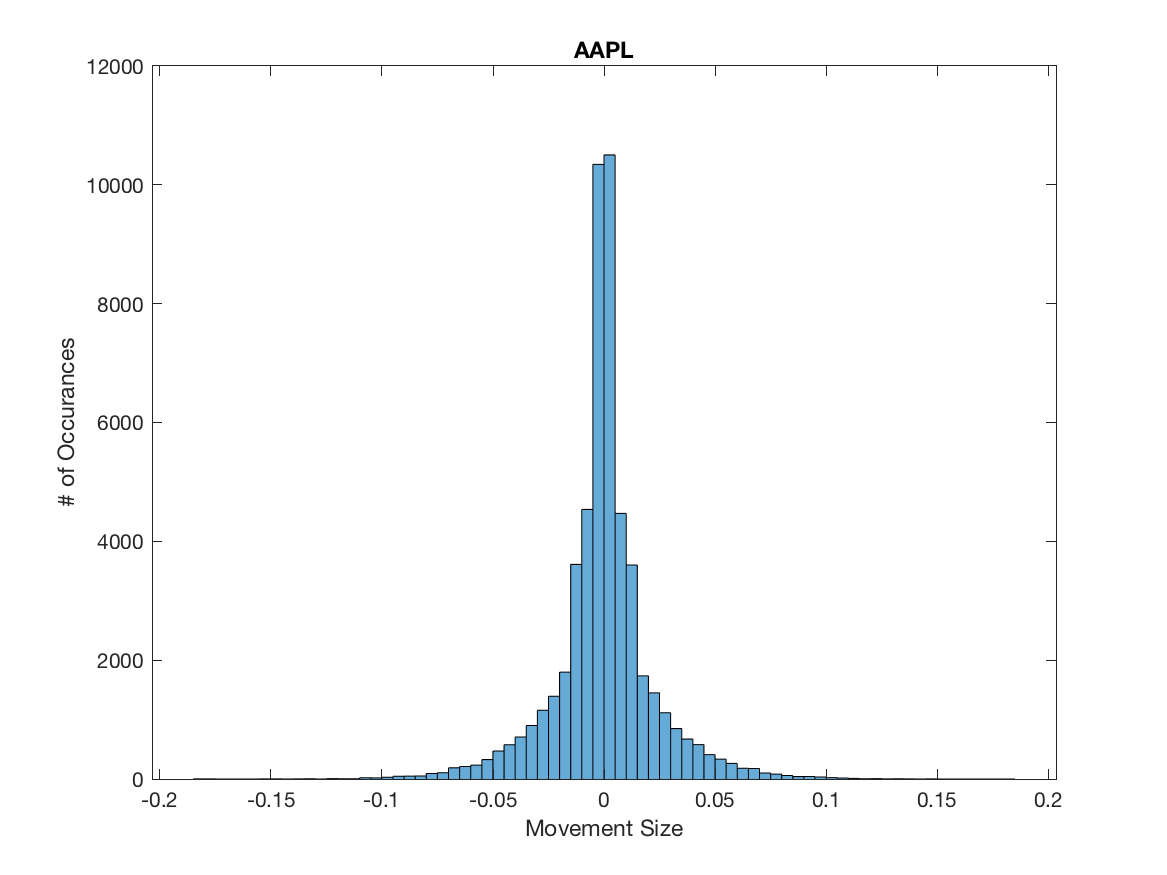
\includegraphics[width=\textwidth, trim = 0 0 0 30, clip]{Tick_Histograms/AAPL_TickHist.png}

\end{subfigure}
\begin{subfigure}[t]{0.49\textwidth}
\captionsetup{labelformat=empty}

\caption{\textbf{AMZN}}
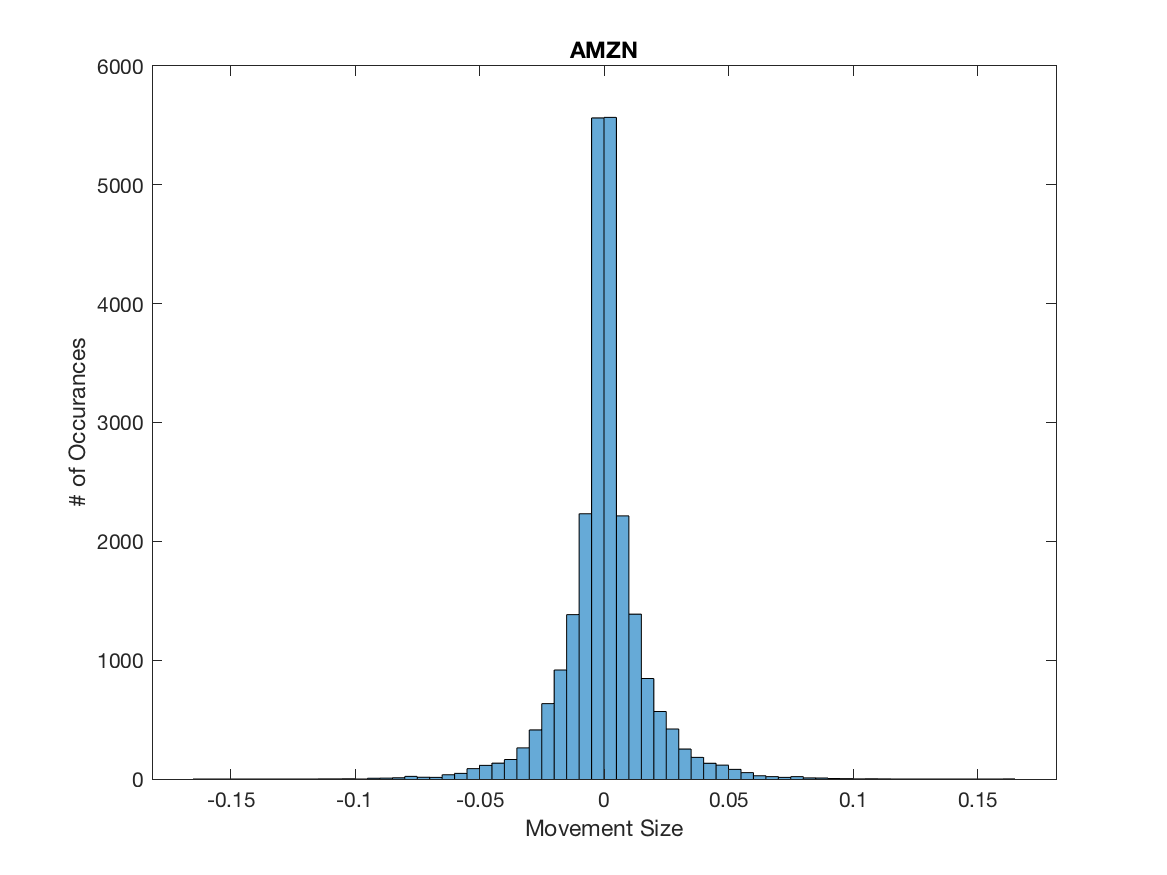
\includegraphics[width=\textwidth, trim = 0 0 0 30, clip]{Tick_Histograms/AMZN_TickHist.png}

\end{subfigure}

\begin{subfigure}[t]{0.49\textwidth}
\captionsetup{labelformat=empty}

\caption{\textbf{GOOG}}
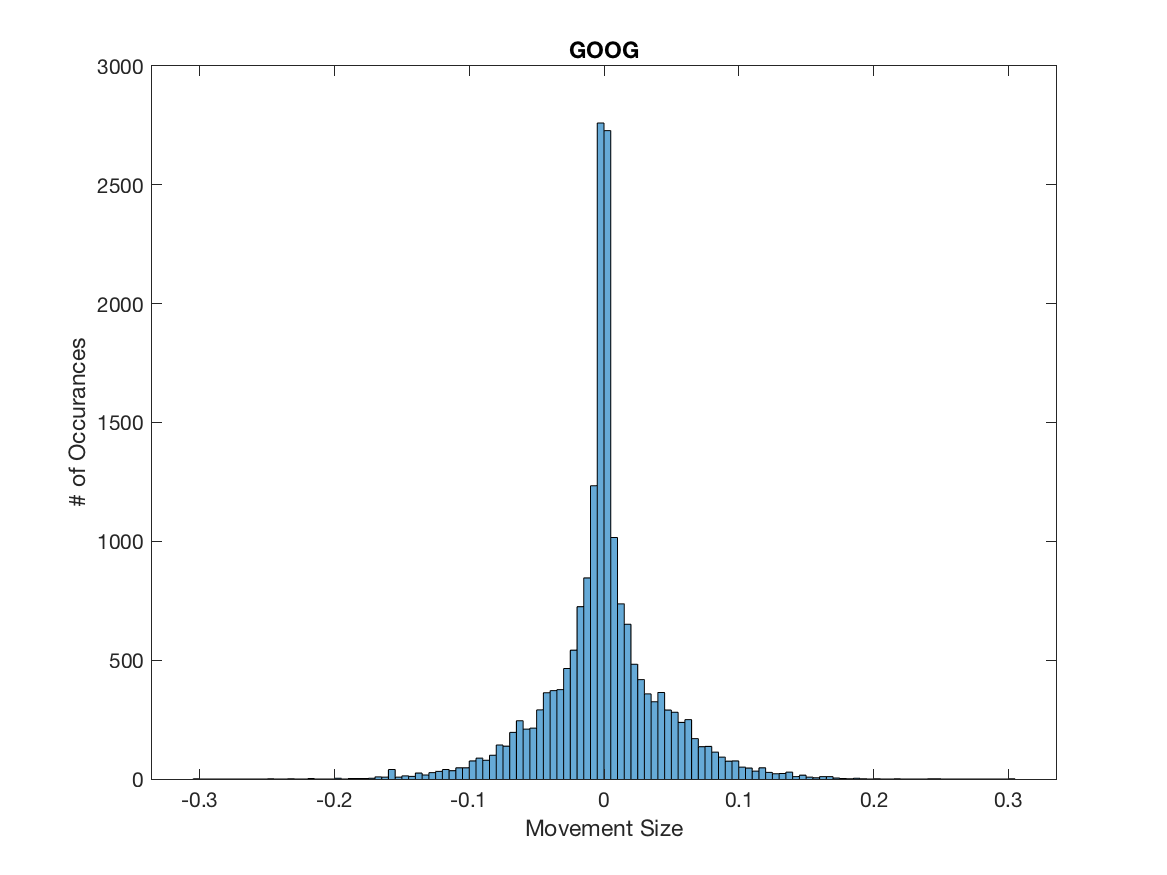
\includegraphics[width=\textwidth, trim = 0 0 0 30, clip]{Tick_Histograms/GOOG_TickHist.png}

\end{subfigure}

\caption{\label{fig:tickhist} We can see clearly that the change in the mid price is often larger than a half tick. These mid price changes make up a significant portion of the actual data, contradicting the assumption needed for the previous model that the mid price changes occur on average at a half tick size.}
\end{figure}

\begin{figure}[htbp]

\centering

\begin{subfigure}[t]{0.49\textwidth}
\captionsetup{labelformat=empty}

\caption{\textbf{AAPL}}
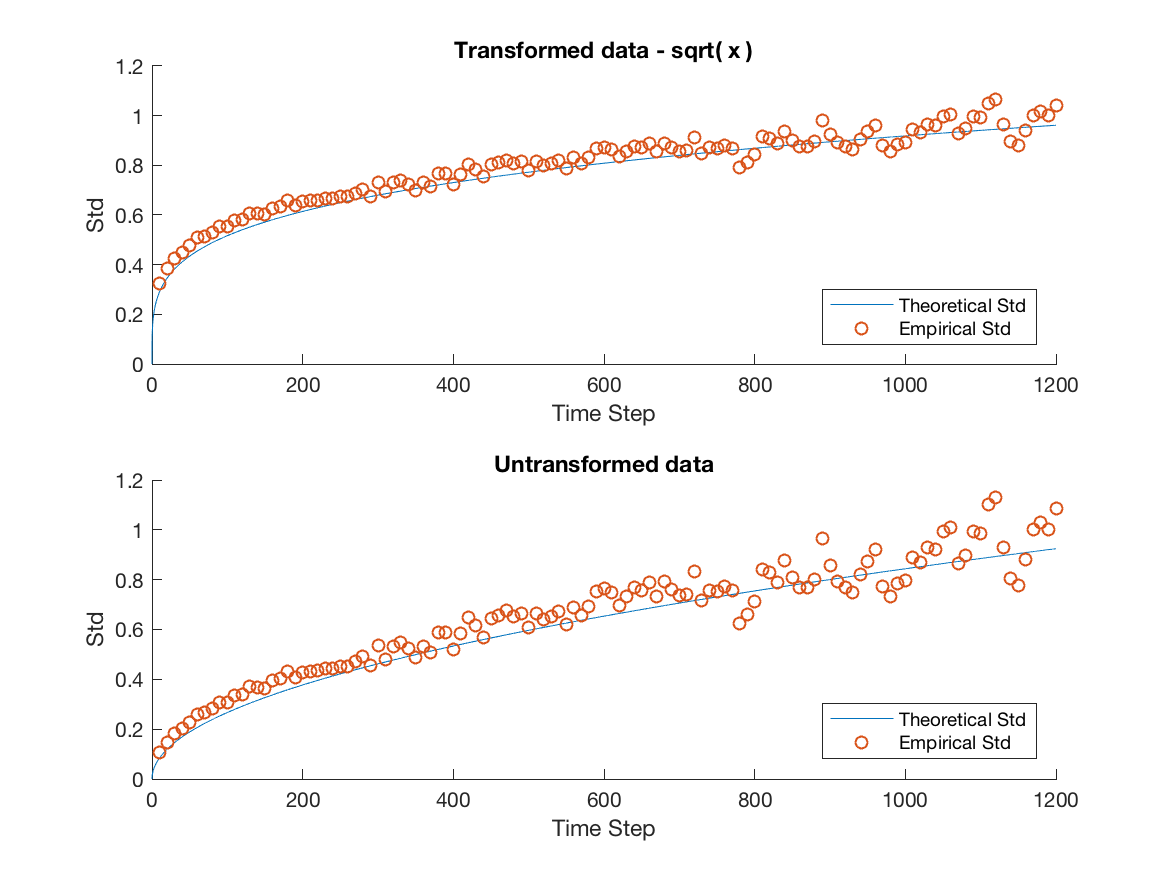
\includegraphics[width=\textwidth]{2SDO_Fit/AAPL_Plot_GCHP2SDO_21600.png}

\end{subfigure}
\begin{subfigure}[t]{0.49\textwidth}
\captionsetup{labelformat=empty}

\caption{\textbf{AMZN}}
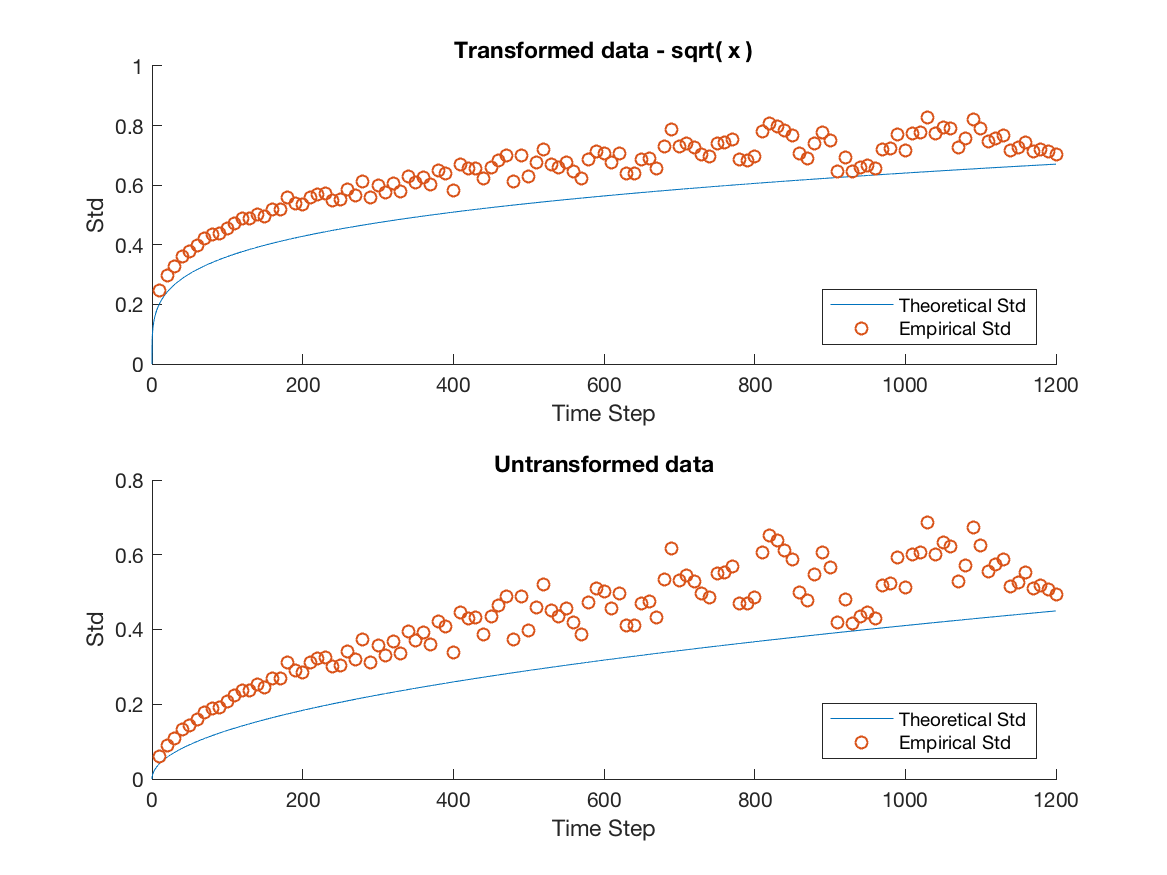
\includegraphics[width=\textwidth]{2SDO_Fit/AMZN_Plot_GCHP2SDO_21600.png}

\end{subfigure}

\begin{subfigure}[t]{0.49\textwidth}
\captionsetup{labelformat=empty}

\caption{\textbf{GOOG}}
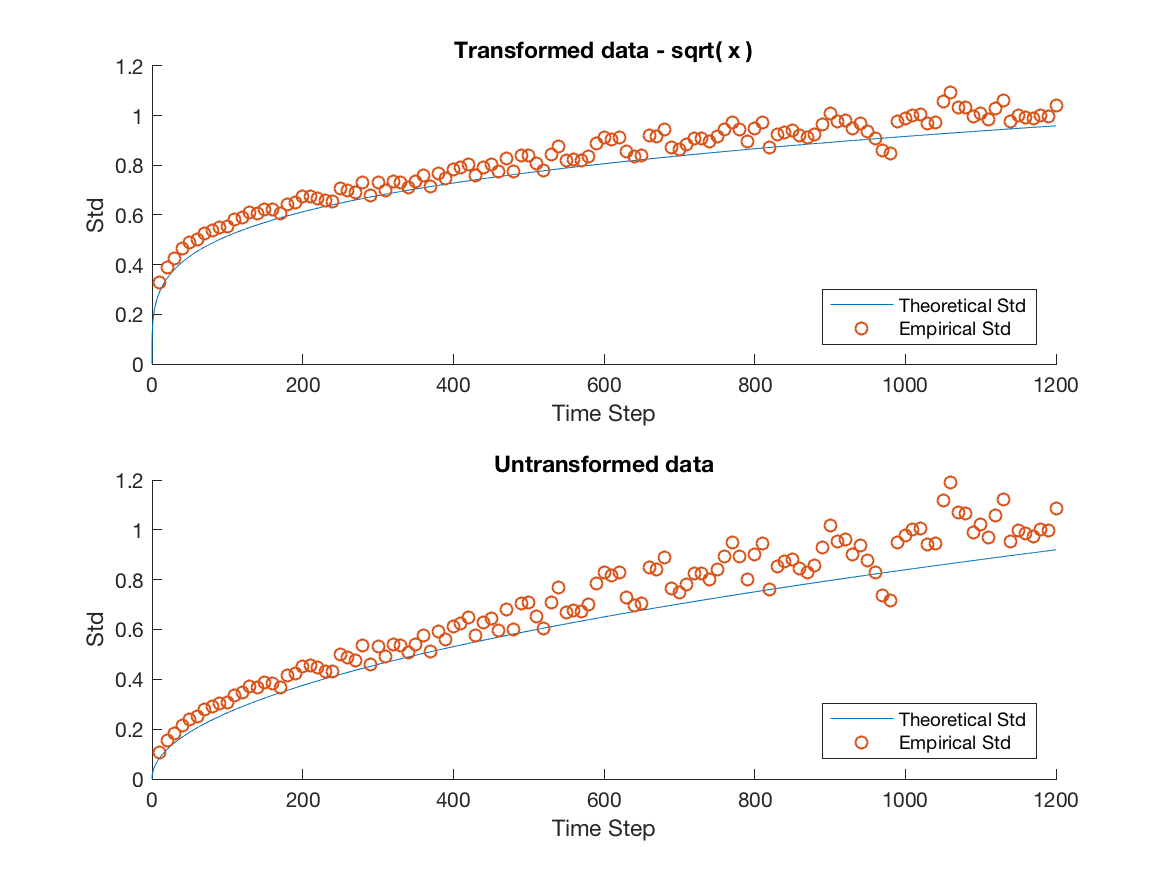
\includegraphics[width=\textwidth]{2SDO_Fit/GOOG_Plot_GCHP2SDO_21600.png}

\end{subfigure}

\caption{\label{fig:2SDOfit} A comparison of the empirical standard deviation for a fixed window size $n$ to the theoretical standard deviation for AAPL, AMZN and GOOG using the 2 state dependent order model. We have plotted the empirical standard deviation for all $n$ from 10 seconds to 20 minutes in step sizes of 10 seconds. Each empirical standard deviation corresponds to a single point in the scatter plot and the plotted curve corresponds to the predicted theoretical value. Visually there is a significant improvement for all stocks, although the theoretical standard deviation for AMZN is still underestimating the empirical variability.}

\end{figure}

\begin{figure}
    \centering
    
    \caption*{\textbf{AMZN}}
    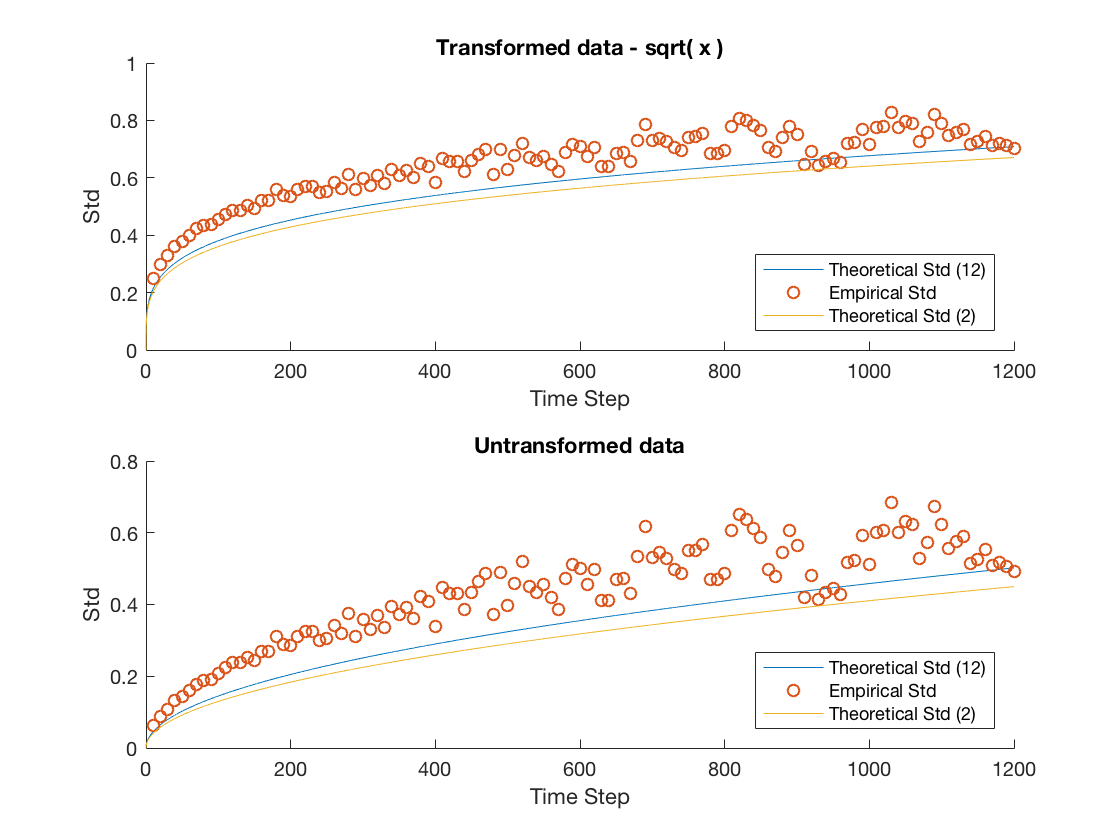
\includegraphics[width=\textwidth]{N_State_Plots/AMZN_N_State.png}
    
    \caption{\label{fig:AMZN_data} We consider the N-state model for AMZN discussed previously in the paper. While there is a slight improvement against the original fit, the model still struggles to perfectly predict the variability in the mid price changes of our data. Comparing the mean residuals, the 2-state model discussed before has mean residual $0.0208$ while our 12-state Markov chain brings that down to $0.0125$. Considering an even larger Markov chain with 24-states we are only able to obtain a meager improvement to $0.0123$, suggesting that there is some underlying variance in the mid price process not captured by our model.}
    
\end{figure}

\end{document}